\documentclass[border=10pt]{standalone}
\usepackage{circuitikz}
\usepackage{tikz}
\usetikzlibrary{calc, positioning, arrows.meta}

\begin{document}
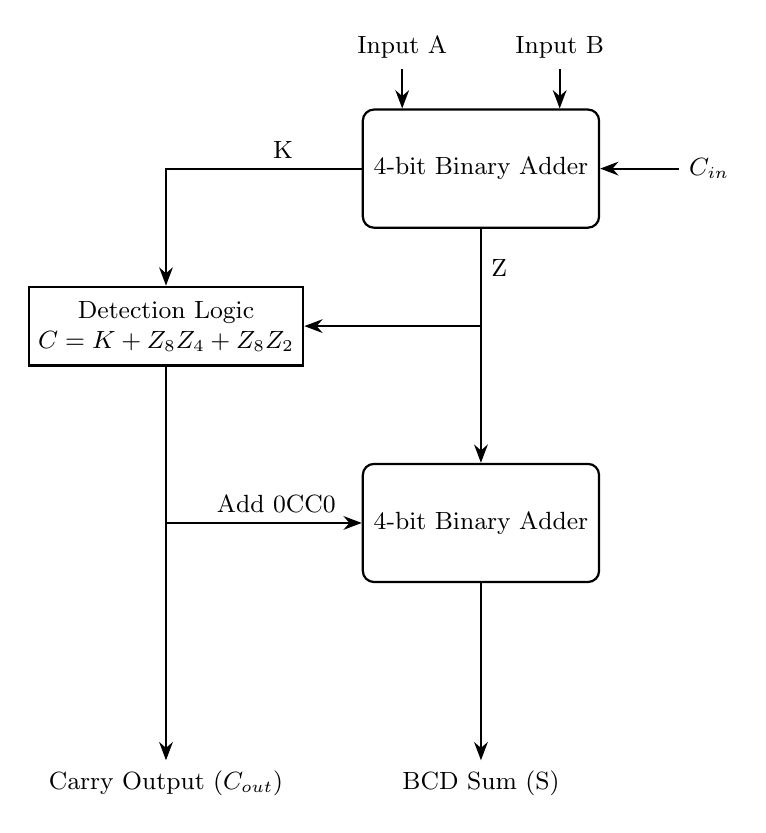
\begin{tikzpicture}[
    >=Stealth, 
    thick, 
    font=\small,
    block/.style={draw, rectangle, minimum height=1.5cm, minimum width=3cm, fill=white, align=center, rounded corners},
    logic/.style={draw, rectangle, minimum height=1cm, minimum width=2cm, fill=white, align=center}
]

    % First Binary Adder
    \node[block] (adder1) at (0, 6) {4-bit Binary Adder};
    
    % Inputs
    \draw[->] ($(adder1.north) + (-1, 0.5)$) node[above] {Input A} -- ($(adder1.north) + (-1, 0)$);
    \draw[->] ($(adder1.north) + (1, 0.5)$) node[above] {Input B} -- ($(adder1.north) + (1, 0)$);
    \draw[<-] (adder1.east) -- ++(1, 0) node[right] {$C_{in}$};

    % Adder 1 Outputs (Z) - Represented as a bus
    \path (adder1.south) -- ++(0, -1) coordinate (z_bus);
    \node[right] at ($(z_bus) + (0, 0.5)$) {Z};
    \draw(adder1.west) -- ++(-1, 0) coordinate (k_out) node[above] {K};
    
    % Correction Logic Block
    \node[logic] (detect) at (-4, 4) {Detection Logic\\$C = K + Z_8Z_4 + Z_8Z_2$};
    
    % Connections to Detection Logic (Abstracted)
    \draw[->] (k_out) -| (detect.north);
    \draw[<-] (detect.east) -- (detect.east -| z_bus);

    % Second Binary Adder
    \node[block] (adder2) at (0, 1.5) {4-bit Binary Adder};
    
    % Z Input to Adder 2
    \draw (adder1.south) -- (z_bus) [->] -- (adder2.north);
    
    % Correction Value (0110 or 0000)
    % We show this coming from the side or conceptually controlled by C
    \coordinate (c_in_2) at ($(adder2.west) + (-1, 0)$);
    
    % Output Carry
    \draw[->] (detect.south) -- ++(0, -5) node[below] (CO) {Carry Output ($C_{out}$)};
    
    % Use C to control the second input to Adder 2 (conceptually)
    \node[above left][xshift=+0.8cm] at (c_in_2) {Add 0CC0};
    \draw[->] (detect.south) |- (c_in_2) -- (adder2.west);
    
    % Adder 2 Output (S)
    \draw[->] (adder2.south) -- ++(0, -2.25) node[below] {BCD Sum (S)};

\end{tikzpicture}
\end{document}
